\subsection{AST\@: Abstract Syntax Tree}

Abstract Syntax Trees henceforth denotes AST, are tree diagrams used to represent
the abstract syntactical structure of a formal language. This is often used when 
writting compilers or other language parsing software.

In the above given example $ 2 * 4 + 5 $ can be expanded into an AST in the following
way.

\begin{figure}[h]
  \centering

  \usetikzlibrary{positioning}
  \tikzstyle{ASTNode} = [draw, circle]
  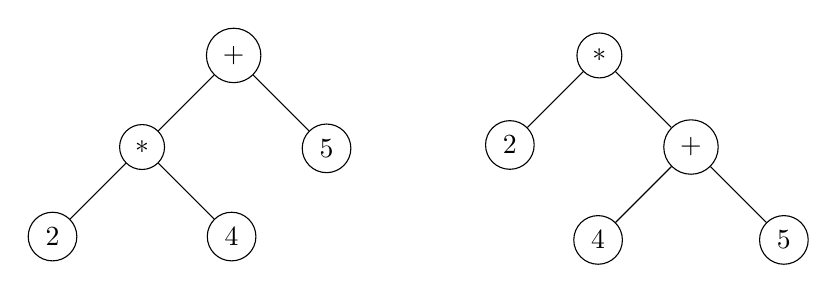
\begin{tikzpicture}[node distance = 1cm, edge/.style={link}]

    \node[ASTNode] (root) {$+$};
    \node[ASTNode] (left) [below left = of root] {$*$} edge (root);
    \node[ASTNode] (right) [below right = of root] {$5$} edge (root);
    \node[ASTNode] (left-left) [below left = of left] {$2$} edge (left);
    \node[ASTNode] (left-right) [below right = of left] {$4$} edge (left);

    \node[ASTNode, node distance = 4cm] (root2) [right = of root] {$*$};
    \node[ASTNode] (left2) [below left = of root2] {$2$} edge (root2);
    \node[ASTNode] (right2) [below right = of root2] {$+$} edge (root2);
    \node[ASTNode] (left2-left2) [below left = of right2] {$4$} edge (right2);
    \node[ASTNode] (left2-right2) [below right = of right2] {$5$} edge (right2);
  \end{tikzpicture}
  \caption{AST showing how one expression can lead to two different result.}%
  \label{fig:AST_Ambiguity}
\end{figure}

The above \autoref{fig:AST_Ambiguity} shows how a simple expression can be ambigous
and this is where grammar rules come into the picture, they tell us how to sort out 
these ambiguities. 
